\section{Model estimation and selection}

\newpage
\section{Data}
\label{section: Data}
In this chapter, the data used to uncover the economic regimes are introduced. A variety of different index will be described, however, the application of them will be specified in subsequent analysis. Initially, decisions related to time horizon and optimal observation frequencies are discussed along with a assessment of which financial data that best captures changing regimes. Once the index data has been introduced and reviewed its distributional and temporal properties are explored in section \ref{subsection: distributional properties} and \ref{subsection: temporal properties}. The objective of the chapter is thus to provide an overview of the data that serves as potential usage for regime detection along with its statistical properties. It should be noted that other indices could have been included, hence the chapter is not intended to be collectively exhaustive. 

\subsection{Time horizon and frequency of data}
\label{subsection: Data frequency}
When utilising financial market data to uncover economic regime changes, a natural questions arises in terms of which data frequency to use. As described, the objective of DAA is to rebalance the portfolios once a regime shifts has occurred, hence if the regime detection relies on too infrequent data, there is a high probability that several regime shifts will remain hidden. As such, data frequencies longer than a month is not considered. Furthermore, as previously mentioned, macroeconomic data is widely available, thereby contributing to its popularity, however, the data is typically characterised by a data frequency of months or even quarters. Therefore, the data frequency of macroeconomic variables propose a challenge, as historic events has shown that economic regime changes can happen swiftly, evident by the recent COVID-19 recession. As such, monthly data compared to e.g. daily data, greatly increases the risk of slow and insufficient detection of economic regime shifts.
 
Despite of the reasoning just outlined, it should be noted that the use of daily data presents some challenges as well. This is due to the fact that daily returns contain a lot of noise and extreme observations, which are evened out on a monthly basis. Consequently, long-horizon returns tend to be more closely approximated by a Gaussian distribution than returns for short-horizon (Campbell et al. 1997). As such, short-term data frequencies complicates the modeling significantly, which can lead to sporadic predictions and less persistence. In addition, the use of daily return frequencies makes the aforementioned link to macroeconomic data more difficult to justify, and therefore it becomes challenging, from a macroeconomic perspective, to argue that economic regime shifts occur since there is no tangible macroeconomic evidence to support this before the data gets collected and released. Despite of the complications associated with short-term data frequencies, the arguments for considering daily as opposed to monthly data frequencies are compelling. 

Furthermore, despite the aforementioned issues with sporadic predictions due to daily data frequencies, Bulla et al. (2011) argued that by relying on daily data it becomes feasible to apply filters that increase confidence whenever a regime change has been detected. As such, research cements the possible of implementing a waiting scheme, in which the portfolio manager would wait several days, when a regime shifts has been detected, before changing the portfolio allocation, thereby minimizing the risk of re-allocating capital based on a wrong signal. In addition, the use of MPC makes daily data frequencies more justified, since it is not possible to make better return predictions for the assets than their long-term average. As such, looking only a limited number of days into the future is not just an approximation necessary to make the optimization problem computationally feasible, it is also reasonable due to the nature of financial returns.

Bulla et al. (2011) further argued that the use of daily data frequencies increases the amount of data available for markets characterised by a short lifetime, however, many financial indices are old and for these older indices monthly data is more available than daily data. Unsupervised machine learning models, such as HMMs, require large amounts of data to be trained in order to achieve a desired and comfortable level of predictability, and as such, the usage of these heavy data-driven models serve as an argument for relying on monthly data as opposed to daily data. Yet, this thesis favors early detection, due to the reasoning outlined above. As a result, daily data, will be used in the analysis. Lastly, the optimal time horizon used for training the model is debatable, however, it should at least span the time required for a financial cycle to unfold in order to include the performance of DAA strategies in several economic environments. Furthermore, it should be acknowledged that, the longer the data horizon the more questionable it becomes whether stationarity of the data-generating process can be assumed (Bulla et al. 2011).

The following sections will include details on selected indices used for training the hidden Markov models, in order to uncover whether different indices lead to similar model parameters and performance across DAA strategies. 

\subsection{The MSCI}
\label{subsection: MSCI Index}
The MSCI World Index captures large and mid cap representation across 23 Developmed Markets (DM) countries. As such, the difference compared to the well-known MSCI ACWI Index is the exclusive weight on assets from developed economies. With 1,600 constituents, the index covers approximately 85\% of the free-float-adjusted market captilization in each country. The weights across country and sectors are shown in figure XXXXY as of November 2020. The historical development of the index is depicted in figure \ref{fig:MSCI_index}. 
 
\begin{figure}[H] 
    \centering
    
\includegraphics[width=0.5\textwidth]{analysis/data_description/images/MSCI_index.png}
    \caption{Development MSCI.}
    \label{fig:MSCI_index}
\end{figure}

%##### INDSÆT FIGUR AF Sector og region focus ####### # VIS split

The inclusion of the MSCI World Index is based on the fact that it is a global index, and thus should capture the economics trends across geographies. As such, the thesis treats it as a baseline index in terms of uncovering economic-regimes. Although it is a world index, North America makes up almost 2/3 of the index, however, this makes sense from an economic perspective since the U.S. economy serves as a fundamental indicator of how the remaining world economy is progressing. Furthermore, the information technology sector is by far the largest sector in the index, since it accounts for approximately 22\% of the overall allocation as per figure XXXXX. It should be noted that the weights are a snapshot in time, hence they are constantly changing. 

\begin{table}[H]
\caption{Summary statistics for the daily MSCI log-returns.}
\centering
\begin{tabular}{c c c c c c c c c} 
\hline\hline
Observations & Mean & STD & Skewness & Excess Kurtosis & Min & Max & First ACF & Annual SR \\
\hline
12,941 & 0.0003 & 0.0087 & -0.6521 & 10.8819 & -0.1044 & 0.0909 & 0.1337 & 0.4854 \\
\hline
\end{tabular}
\label{tab:summary_stats_MSCI}
\end{table}

Table \ref{tab:summary_stats_MSCI} shows the first four central moments together with the minimum and maximum observation, the first-order autocorrelation and the annual Sharpe ratio (SR). The SR is the excess return per unit risk, i.e. the excess return divided by the standard deviation (SD). The first observations originates from 1969-12-31 and the final included observations is the date 2021-02-12. It appears that the daily log-returns for the MSCI World Index are negatively skewed and the distribution is also characterised by being highly leptokurtic as the excess kurtosis is positive. As such, the summary statistics indicate that the log return series for the MSCI World Index, are characterised by the set of stylized facts that are commonly associated with financial returns. The range of the observations has a span of 0.1953, thereby indicating that the index can change significantly in high-volatility periods.    
 
\subsection{The S\&P 500}
The S\&P 500 is a stock index comprising 500 companies from the U.S. which was founded in 1957. The stocks that make up the index are selected by a committee which include representation from all major segments in American industry. As such, contrary to prevailing public sentiment, the index is not simply made up of the 500 largest companies in the U.S. The S\&P 500 Index is a market-capitalization-weighted index in which the 10 largest companies account for 27.5\% of the capitalization of the index as of per December 2020. Figure \ref{fig: SP500_index} showcases the development of the S\&P 500 Index since origination. 
 
\begin{figure}[H] 
    \centering
    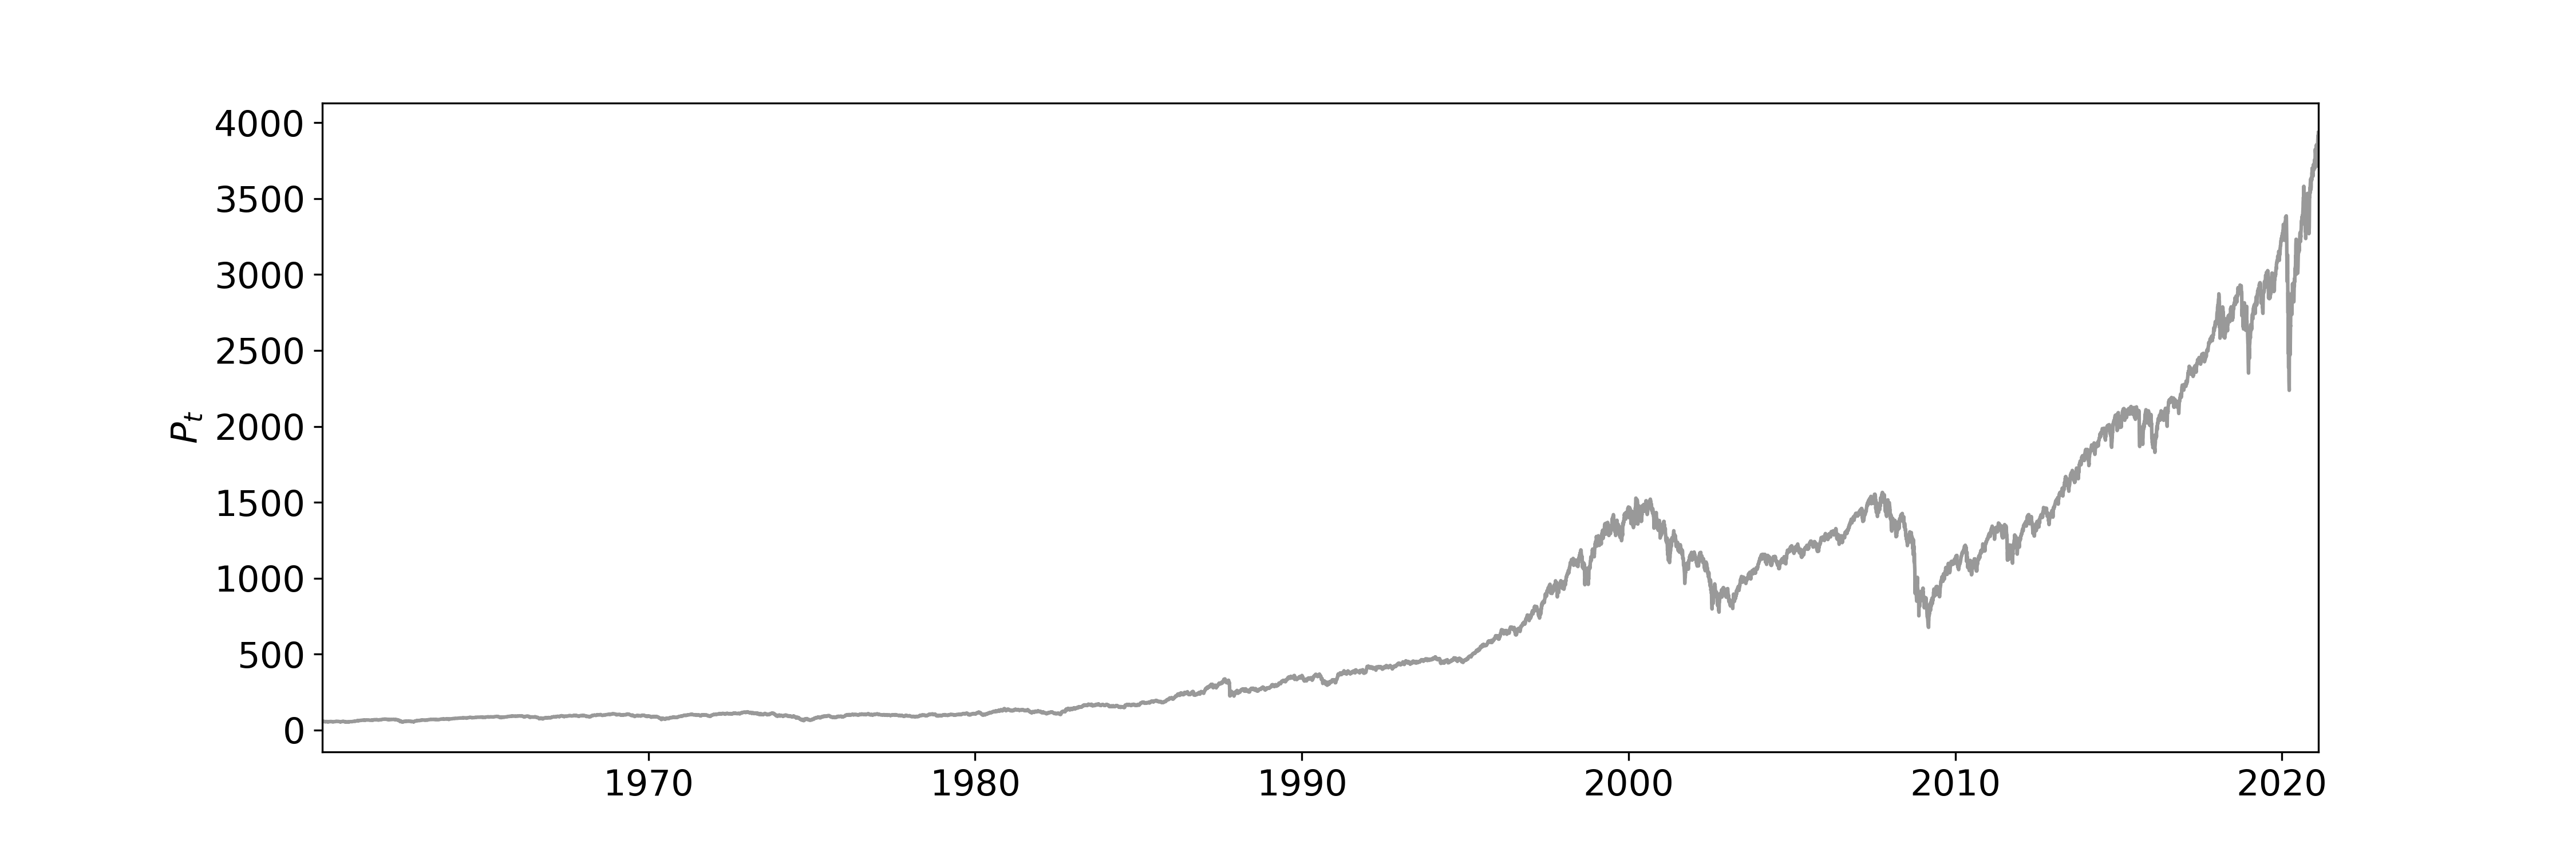
\includegraphics[width=1\textwidth]{analysis/data_description/images/SP500_index.png}
    \caption{Development S\&P 500.}
    \label{fig: SP500_index}
\end{figure}

As is evident from figure \ref{fig: SP500_index} the 44 year data period has been impacted by the major market movements including black monday in 1987 as well as the dot-com bubble of the late 90s and early 2000s. Furthermore the attractive bull market leading up to the GFC has been well-captured by the development of the S\&P 500 Index. Lastly, the long bull market following the GFC as well as the recent COVID-19 correction and rebound appears to be well-captured by the S\&P 500 Index, thereby indicating that it will serve well for model estimation purposes.  

It is unlikely that the recent bullish environment for stocks will continue in perpetuity, since interest rates and inflation, at some point, are likely to start increasing. When that happens, investments towards stocks and indexes can procure short to mid-term monetary losses, however, it is evident from figure \ref{fig: SP500_index} that there appears to be a strong upwards trend historically, thus supporting the argument for capital allocation towards stocks in general.


\begin{table}[H]
\caption{Summary statistics for the daily S\&P 500 log-returns.}
\centering
\begin{tabular}{c c c c c c c c c} 
\hline\hline
Observations & Mean & STD & Skewness & Excess Kurtosis & Min & Max & First ACF & Annual SR \\
\hline
15,385 & 0.0003 & 0.0103 & -1.0353 & 23.8338 & -0.2290 & 0.1096 & -0.006 & 0.4350 \\
\hline
\end{tabular}
\label{tab:summary_stats_S&P500}
\end{table}
 
Compared to the MSCI Index it is evident by table \ref{tab:summary_stats_S&P500} that the daily log-returns of the S\&P 500 encompass similar mean daily returns, although the daily standard deviation is higher. Furthermore, the S\&P 500 Index is more left-skewed, more leptokurtic and the range is much larger at 0.3386. The larger range can primarily be attributed to the Black monday event of 1987 in which the S\&P 500 was much harder impacted relative to the other included indexes. Naturally, these conclusions leads to a lower annual Sharpe Ratio of 0.4350 compared to the MSCI which holds an annual Sharpe Ratio of 0.4854.
 
\subsection{DAX 30}
\label{subsection: DAX 30}
The DAX is a blue chip stock market index comprising the 30 largest listed German companies. It is similar in nature to FTSE 100 and the Dow Jones Industrial Average. The index is included in the analysis in order to get an estimate for, whether the model parameters will change significantly when trained on the DAX as opposed to the aforementioned indexes. As such, the DAX becomes particularly interesting since its composition of a small number of firms and a restrictive geographical focus on Germany means that it might not necessarily represent the vitality of the economy as a whole. 

\begin{figure}[H] 
    \centering
    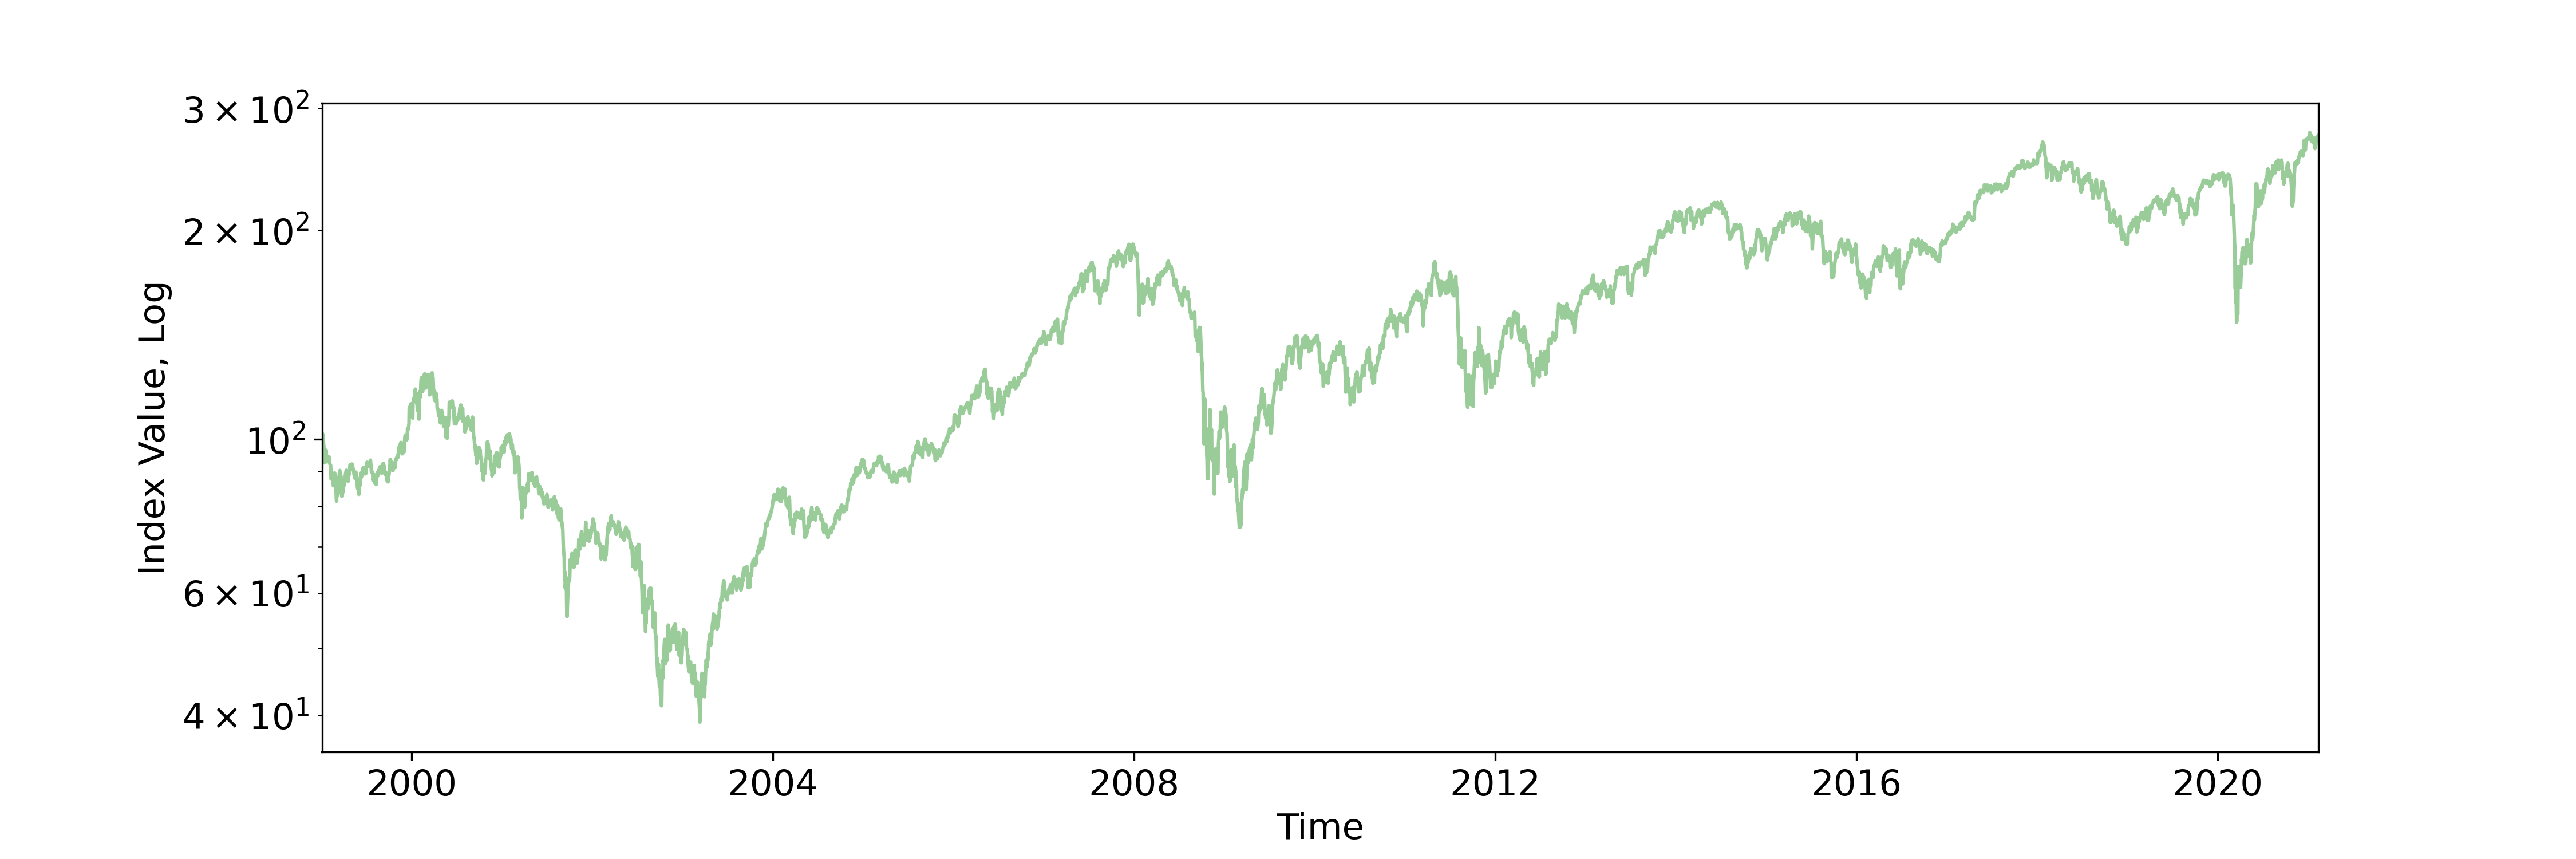
\includegraphics[width=1\textwidth]{analysis/data_description/images/DAX_index.png}
    \caption{Development DAX 30.}
    \label{fig: DAX_index}
\end{figure}

As is evident by figure \ref{fig: DAX_index}, the availability of daily data is significantly shorter compared to the MSCI World and the S\&P 500 Index. This is primarily due to the fact that the DAX 30 was originated in the late 1987. However, figure \ref{fig: DAX_index} also showcases that recent financial bear markets such as the dot-com bubble of the early 2000s, the GFC of 2008 as well as the COVID-19 rebound in Q1/Q2 2020 are well captured by DAX 30 Index. 

Since January 2006, the index is refreshed every second, however, the thesis will continue to rely on daily data frequencies as discussed in section \ref{subsection: Data frequency}. The index is capitalization-weighted and holds a total market capitalization of 1,017.7 billion EUR as of 21st of September 2020. In response to the recent accounting scandal related to Wirecard, Deutshce Börse announced an expansion of the DAX 30 to include 40 members. The expansion is set to occur in the third quarter of 2021.

\begin{table}[H]
\caption{Summary statistics for the daily DAX log-returns.}
\centering
\begin{tabular}{c c c c c c c c c} 
\hline\hline
Observations & Mean & STD & Skewness & Excess Kurtosis & Min & Max & First ACF & Annual SR \\
\hline
5,613 & 0.0002 & 0.0159 & -0.1869 & 2.8115 & -0.1394 & 0.1257 & 0.0146 & 0.1839 \\
\hline
\end{tabular}
\label{tab:summary_stats_DAX}
\end{table}

As highlighted by table \ref{tab:summary_stats_DAX}, the DAX Index contains much fewer observations compared to the MSCI World and S\&P 500 index. Furthermore, the DAX has similar mean daily returns although the standard deviation is the highest among the selected indices. However, the DAX is less negatively skewed and exhibit the lowest degree of leptokurtotic among the selected indexes. However, the high standard deviation naturally leads to a much lower Sharpe Ratio compared to the other indices at 0.1839.

\subsection{Distributional properties}
An overview of the development for the three selected indexes have been plotted in figure (ref til figur hvor udvikling plottes i samme graf), however, the indexes have been adjusted so that they all comprise the same amount of observations. This means that the first observation is from 04-01-1999 and the last observation is 12-02-2021. 

%%%% INDSÆT FIGURE hvor alle index er vist på samme graf (evt. inkluder yields)

From an overall return perspective it is evident that the S\&P 500 Index has performed better than the other alternatives. Interestingly, the S\&P 500 Index only recovered from the dot-com bubble a few months prior to the financial crisis of 2008, yet it was severely impacted by the GFC. In the period following the financial crisis the S\&P 500 has been performing increasingly well resulting in an upward-trajectory until the recent COVID-19 correction, after-which the index reached the present all time high values. 

The MSCI World Index appears to have a more stable trajectory with less volatile movements both compared to the S\&P 500 and the DAX 30. Despite this, the MSCI World Index generally trended in the same direction as the S\&P 500,
but in some periods the range between the two indices widened. For example,
it appears that the MSCI World and S\&P 500 Index trended in close correlation in the period from 1999 to 2015, however, from 2015 to 2021 the two indices have drifted apart. Furthermore, it appears that the S\&P 500 has become increasingly more volatile over the period 20015-2021, particularly evident by the recent COVID-19 rebound in which the drawdown of the S\&P 500 was much more extreme compared to the MSCI World.  

The DAX 30 performed particularly well in the period following the dot-com bubble, however, during 2008 and 2009 the GFC severely impacted the index, thereby bringing it down to the respective levels of the S\&P 500 and MSCI World. As concluded in section \ref{subsection: DAX 30} the DAX was characterised as the most volatile, which is also evident by figure (ref til kombineret figur) which showcases that the DAX indeed appears to have a higher volatility. From 2006 to 2017 the DAX Index has consistently been at higher index levels compared to the other indices until the S\&P 500 caught up by breaking its all time high in 2019. An overview of the summary statistics for each index is listed in table \ref{tab:summary_all}.

\begin{table}[H]
\caption{Summary statistics for the daily log-returns of the three indices}
\centering
\begin{tabular}{c c c c}
\hline
 & MSCI World & S\&P 500 & DAX 30 \\
\hline 
Observations & 12,941 & 15,385 & 5,613 \cr Mean & 0.0003 & 0.0003 & 0.0002 \cr STD & 0.0087 & 0.0103 & 0.0159 \cr Skewness & -0.6521 & -1.0353 & -0.1869 \cr Excess Kurtosis & 10.8819 & 23.8338 & 2.8115 \cr Min & -0.1044 & -0.2290  & -0.1394 \cr Max & 0.0909 & 0.1096 & 0.1257 \cr Annual SR & 0.4854 & 0.4350 & 0.1839
\\
\hline
\end{tabular}
\label{tab:summary_all}
\end{table}

\subsubsection{Log Returns}
As evident by figure (ref til index udvikling) the series are not stationary since the mean values are growing and when zooming in on local periods there appears to be strong trends. As such, a transformation is needed to obtain stationary time-series. In cases where the series is characterised by growing means and local trends a log-transformation will narrow the gap between the indices and taking the first difference will eliminate the growing mean values. This results in the log-returns being derived as $r_t = log(P_t) - log(P_{t-1})$, where $P_t$ is the adjusted closing price of the index on day $t$ and log is the natural logarithm. For daily returns less than 10\%, log returns are a good approximation to the discrete return, as it is the first order Taylor approximation.

Table \ref{tab:summary_all} showcases the summary statistics for the daily log-returns of the selected indices together with the annual Sharpe ratio and the JArque-Bera (JB) test statistic. As already noted the distributions are left skew and leptokurtic. The critical value for the Jarque–Bera test statistic at a 99.9\% is 14.13 Thus, the Jarque–Bera test strongly rejects the normal distribution for all three indices.  

In addition, it is evident from the plot of the kernel disnity functions in figure ref til figur (de billeder med normalfordeling vs. empirisk fordeling) that the log returns series are characterised by excess kurtosis relative to a Gaussian distribution. As such, there is too much mass centered around the mean and in the tails compared to the Gaussian distribution. The fat left tail implies that using a Gaussian distribution to model returns will underestimate the frequency and magnitude of downside events (Nystrup, 2014). 

%%% INDSÆT FIGUR AF KERNEL PLTOS i.e. normalfordeling vs. empirisk fordeling)

Furthermore, it is evident from figure (ref til kernel plots) that all three indices encompass extreme observations that lie more than 3 standard deviations from the mean. There are 187 observations that deviate more than 3 standard deviations from the mean for the MSCI World index which is way above the expected 39 if the series followed a Gaussian distribution. Out of these, 74 observations are located in the right side of the tail while the remaining 113 are located in the left tail. This phenomenon that large drawdowns occur more often than similar large upwards movements is well researched and known as the gain/loss asymmetry (Cont, 2001). In addition, it should be noted that since the MSCI World contains 12,941 observations, it only takes a few outliers to reject that the series follow a normal distribution. However, as noted by Cont (2001), financial returns are characterised by a large degree of extreme observations compared to the Gaussian distribution, which is evident by the large excess kurtosis from table \ref{tab:summary_all}.

Lastly, it is important to note the subtle distingshion between outliers and extreme observations since extreme observations deviate considerably from the group mean, yet they may still hold meaningful information hence they should not be disregarded.
Since extreme events happen in live markets the observation that they create should be included in the model estimation in order for the model be as realistic as possible.

%%% INDSÆT FIGUR AF LOG RETURNS FOR ALLE INDICES.


\label{subsection: distributional properties}

 
\subsection{Temporal properties}
\label{subsection: temporal properties}
It is evident by the plot of the log returns for the different indices in figure (ref til figure) that the log returns are characterised as mean stationary, since they fluctuate around a constant mean level close to zero for all three indices. Despite this, the log-returns series for all three indices are seen to be more volatile in some periods. The effect that large prices movements tend to be followed by other large price movements, but not necessarily in the same direction, is known as volatility clustering (Cont, 2001). 

Particularly the MSCI World and S\&P 500 index appear to have increasing volatility throughout time, whereas the DAX 30 appears to have similar or slightly contracting volatility levels. This is not surprising as the MSCI World and S\&P 500 index include observations beginning from the 1970s and 1960s respectively. During these times, there were no active derivative markets and much fewer actors had direct access to trading financial instruments. As such, markets were simpler, less risky and thus characterised by an overall lower level of volatility. 

%%%%% INDSÆT billede af ACF og absoloute ACF

The autocorrelation functions (ACFs) for the log-returns and the absolute log-
returns are shown in figure (ref til ovenstående). The black dashed lines make up the bands for the 95\% confidence intervals. The first-order autocorrelation is only significant for the MSCI World index. However, the reader should note that the ACF is time-varying, thus if one were to zoom in on a narrower time-period it is highly probable that the first-order autocorrelation could be significant for all indices. 

The absolute ACFs derived from the log-returns show significant autocorrelation that persists all the way up to lag 100 for all the selected indices. This suggests that financial returns exhibit a memory component, thereby making volatility somewhat predictable. As such, the long memory of the absolute log-returns is closely related to the previously described volatility clustering from figure (ref til figur af log returns).

Conclusively, the reader should note that the correlation among the indices are stronger at the times of high market volatility. This is perhaps not surprising since the indices are made up of stocks, however, it highlights that diversification based on investing in different sectors or geographical areas may not materialize precisely when an investor needs it the most. The impact but most probably be less significant if one were to compare a stock index with a bond index, since the correlation would be lower. Despite the fact that correlations increased in high volatility markets, there are definitely benefits related to diversification between asset classes.